\section{State of the art}
\label{s:Stateoftheart}

The field of soft robotics has gained in interest, in the subsequent sections we will go through some implementations of grippers/manipulators that have been presented.


Mention the fact that there exist different type of grippers in soft robotics thanks to the review of shintake.

\subsection{Soft robotic fingers and hands}
\label{s:SoftRoboticHands}
A very common manipulator in soft robotics is the Robotic Hand. Directly inspired by the large capabilities of the human hand especially the act of grasping. Grasping an object is the act of embracing it with the fingers or arms (Merriam-Webster).Grasping seems to be specific to hand like manipulators, composed often of a palm to which fingers are attached. These can move either independently or simultaneously. Robotic Hands can be regarded sometimes as a very rigid end-effector (e.g. fist), but also as soft (e.g. when handling flowers). We can distinguish precise and fine grasping (a surgeon removing skin tissues), or the use of tools (drills, hammers). The range and order of magnitude of the hand capabilities is large and can go from grabbing a thin hair to catching a football. Various attempts have been made to create robotic hands. Including all the characteristics such as fine sensing, gentleness, robustness, adaptability and in hand re-grasping is extremely challenging. Soft robotic hands are believed to have a simpler control structure and still be very versatile as presented by R. Deimel and O. Brock \cite{deimel2016novel} (Figure~\ref{f:Robotic Hands}). In their work they introduce a robotic hand composed of pneumatic fingers around a soft palm. Testing occurred using the Kapandji test \cite{kapandji1986clinical} showing similar capabilities to a human hand. A more complex design involving though only three fingers was presented by Lael U. Odhner et al. with the iRobot-Harvard-Yale Hand (Figure~\ref{f:Robotic Hands}) \cite{odhner2014compliant}. The fingers can pivot and adapt to the object they intend to grab and manipulate. Softness is not only created by this feature but also through flexible tendons between the phalanges allowing the fingertips to be compliant. It is a good example of a combination between rigid links and soft joints. In industry soft grippers are also presented such as the one from Festo AG \& Co. KG \footnote{Festo: https://www.festo.com/group/en/cms/10221.htm} (Figure~\ref{f:Robotic Hands}). Attention is also brought on improving the design of the fingers alone. Zhu et al. \cite{Zhu} developed a finger with varying stiffness involving multi-layered jamming to increase force capabilities. Many other attempts have been made in this direction \cite{kim2013novel, shan2015rigidity, firouzeh2015soft} but none seems to test the increase in precision and grasp quality when applied to a whole hand.   

\begin{figure}[ht]
\centering
\subfigure[RBO Hand 2]{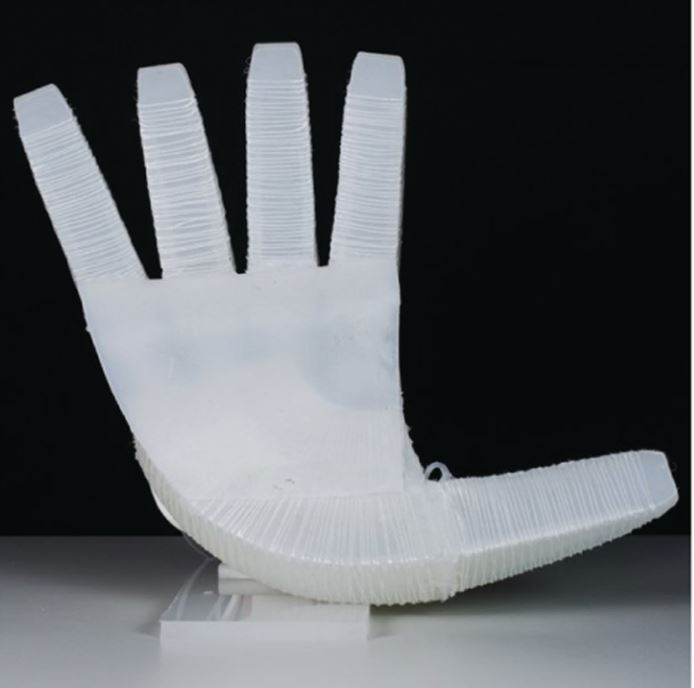
\includegraphics[height=40mm]{Images/rbo_hand2.jpg}}\quad
\subfigure[iRobot-Harvard-Yale]{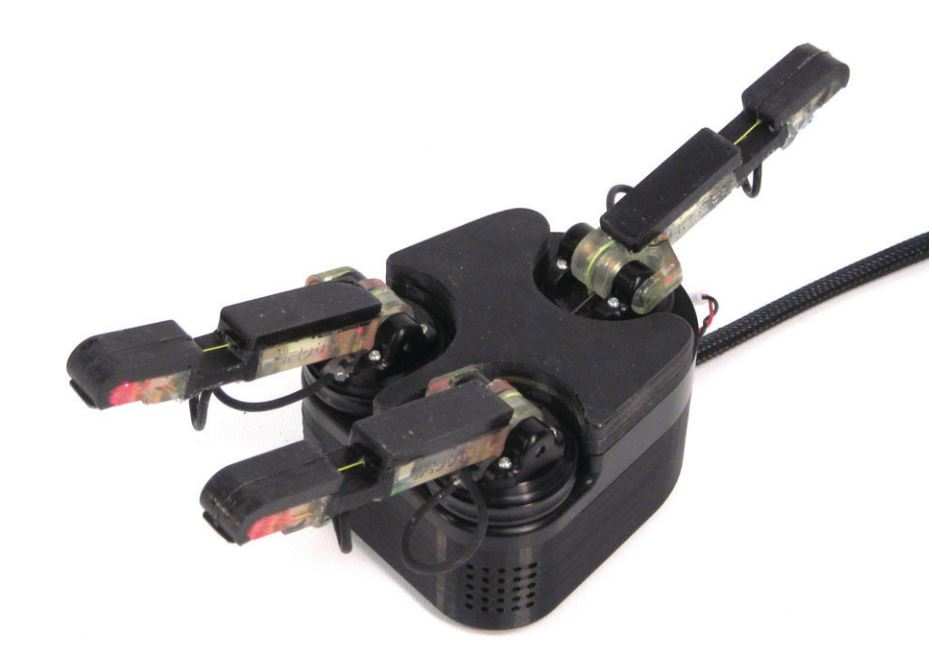
\includegraphics[height=40mm]{Images/compliant_underactuated_hand_for_robot_manipulation.jpg}}
\subfigure[Bellows fingers]{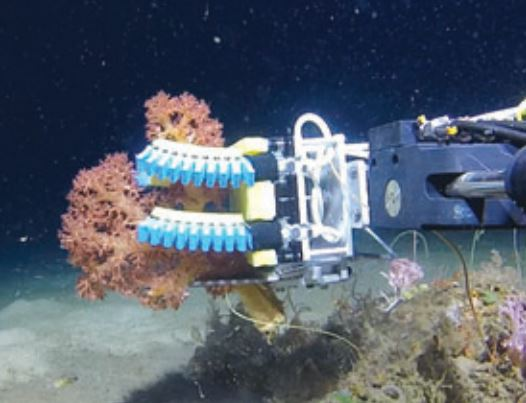
\includegraphics[height=40mm]{Images/deep_sea_hand.jpg}}
\subfigure[Soft industrial gripper from Festo AG \& Co.KG]{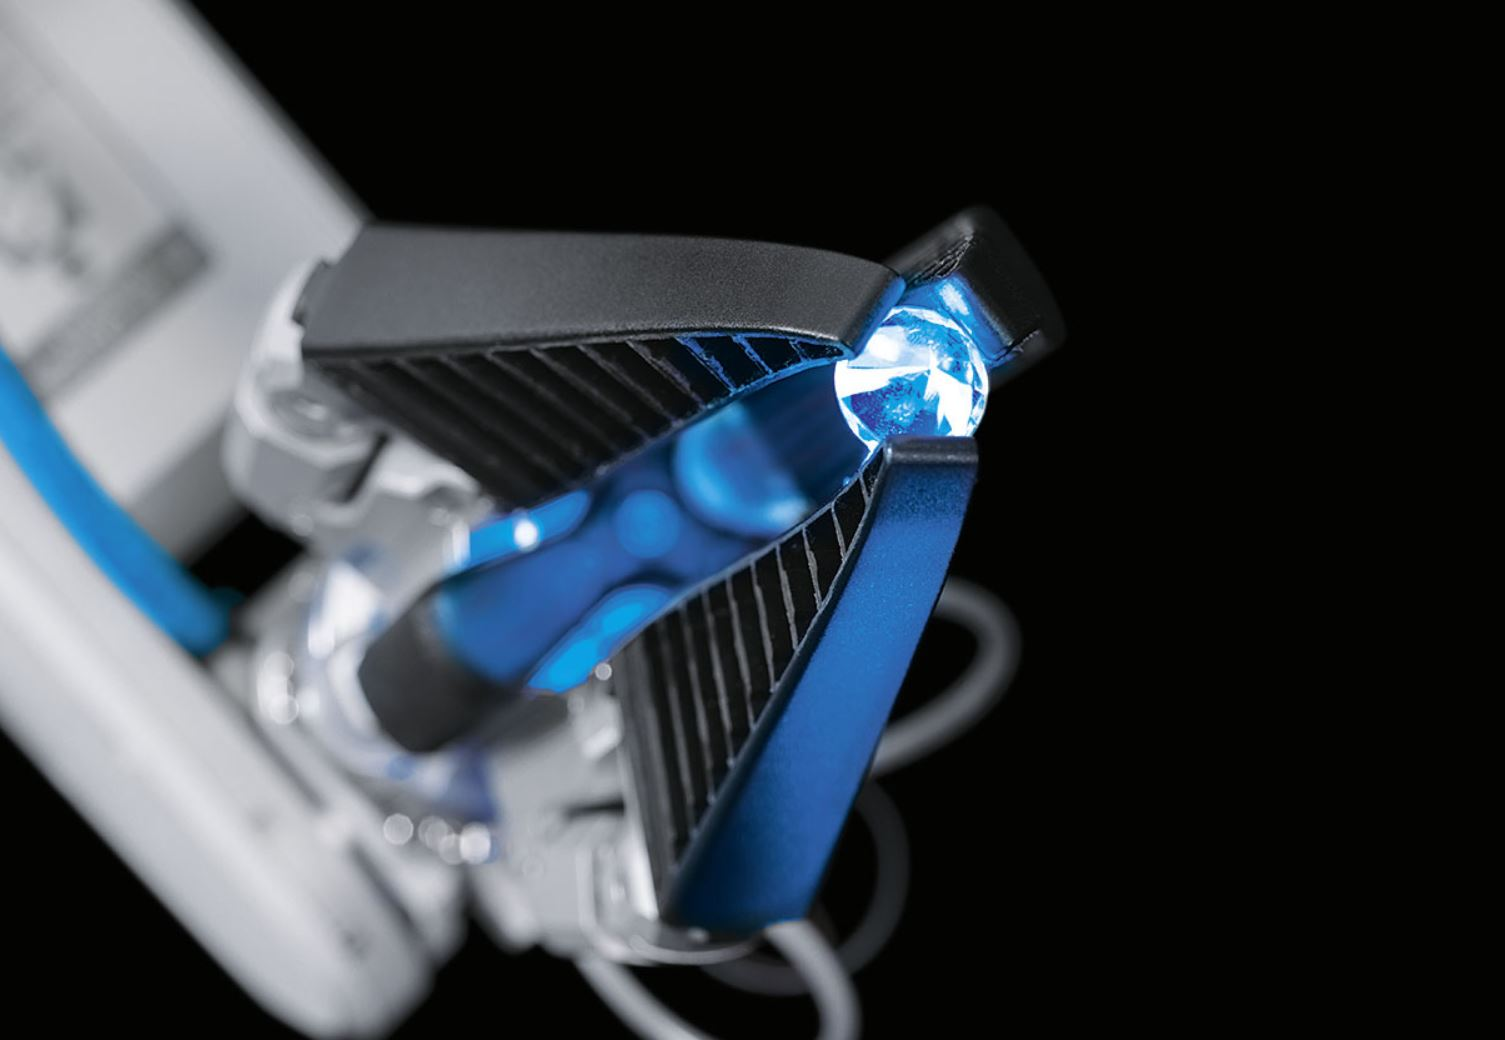
\includegraphics[height=40mm]{Images/festo.jpg}}
\caption[Robotic Hands]{\label{f:Robotic Hands} Different type of robotic hands. (a) The RBO hand is equipped with Pneuflex fingers and is actuated with pressure like the Bellows type finger for deep-sea application. (b) The iRobot-Harvard-Yale hand uses compliant joints which can also rotate.(c) Bellows fingers in deep-sea application. (d) Festo gripper with finray fingers.}
\end{figure}

\subsection{Other soft end-effectors}
\label{s:OtherSoftManipulators}

There exist other robotic grippers that are considered soft and do not take the shape of a hand with fingers placed around a palm. An example of this set up is the jamming gripper presented by Eric Brown et al. \cite{brown2010universal, amend2012positive} . It has the capability to grasp objects by changing the state in which the grains are. The transitioning between liquid-like state and solid-like state occurs through pressure changes. An obvious advantage of such a gripper is its capability to highly adapt to the morphology of the target. It also present a simplified actuation and computation compared to fingers which often are activated individually. However as simple as this solution sounds, there are a few flaws: it can have difficulties grasping objects on soft compliant surfaces.The softness of the surface  will not allow the jamming end to embrace efficiently the target as it will sunk n and not present a surface large enough for the gripper to embrace. A similar idea was developed by S. Li et al. \cite{li2017fluid} which relies also on pressure changes but instead of coffee beans uses internal origami structures. Like a muscle, it will through pressure changes, open or close. Trunk-like end-effectors are also used in grasping tasks. The bellows-type grasper from Galloway et al. \cite{galloway2016soft} is a single finger entangling itself around the target. Compared to the finger described in the same publication, it does not need a palm and can act on its own. 

There exist also several other techniques allowing a soft-touch and a seemingly gentle grasping. Some, for instance, use adhesion in a controlled way. It allows the manipulation of fragile objects since the normal force of the gripper acting on the target object can be reduced by and increase in the shear forces brought by the adhesive properties of the gripper's surface \cite{shintake2016versatile, shintake2018soft} (Figure~\ref{f:Other Effectors}). Shintake et al. \cite{shintake2018soft} distinguish two types of adhesion : electro and gecko adhesion. 

\begin{figure}[ht]
\centering
\subfigure[Jamming gripper]{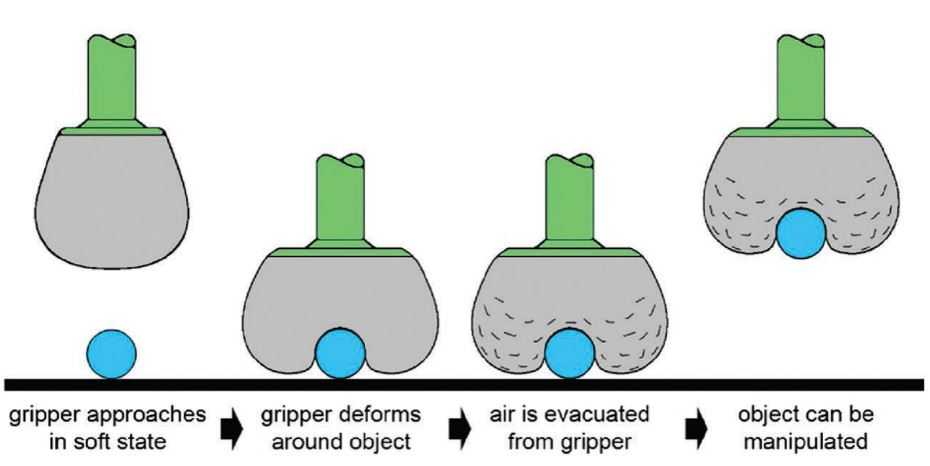
\includegraphics[height=50mm]{Images/jamming.jpg}}\quad
\subfigure[]{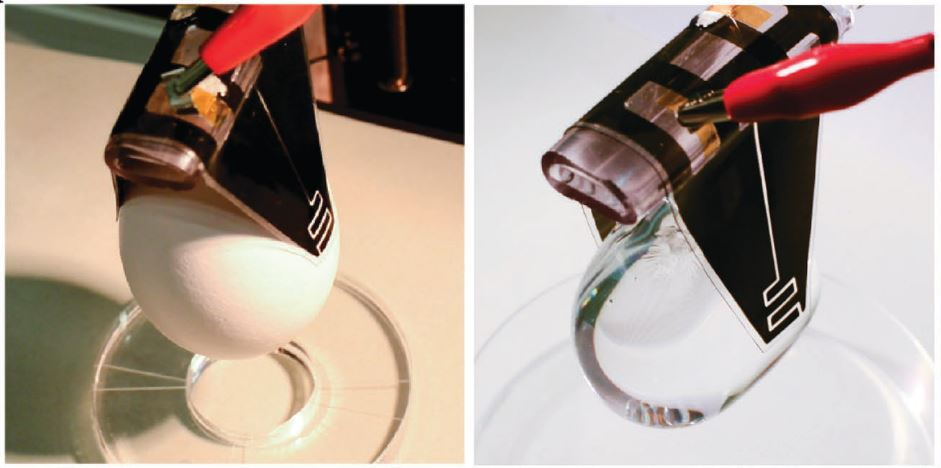
\includegraphics[height=35mm]{Images/electro_adhesion_1.jpg}}\quad
\subfigure[]{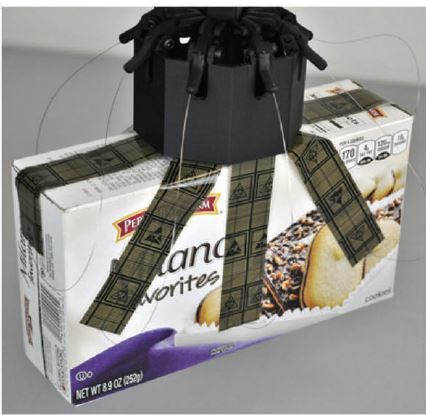
\includegraphics[height=35mm]{Images/electro_adhesion_2.jpg}}\quad
\caption[Other Effectors]{\label{f:Other Effectors} (a) The jamming of grains allows the gripper to seize target objects of various shapes. (b) Example of an electro adhesive gripper grabbing an egg and a water filled balloon.(c) Electro adhesive gripper developped by Grabit Inc.\footnote{Grabit: https://grabitinc.com/products/} }
\end{figure}

\subsection{Testing for robotic end-effectors}
\label{s:TestinginRobotics}

 Measuring the quality of a grasp is not a trivial task for soft robots. As opposed to rigid robotic hands and fingers, the sensing capabilities are restrained. Rigid links have the possibility through reacting forces and servoing to estimate accurately position and other events acting on the system. Sensors backed by accurate path planning as well as state estimation can help create a precise motion. In soft-robotics similar metrics can be applied for measuring precision.  However when it comes to measuring adaptability and gentleness, there is no unified and standardized method. It appears that testing for robotic end-effectors is disparate. Some groups use balloons with thin membranes, eggs \cite{shintake2016versatile}, tubes \cite{galloway2016soft} or other objects \cite{odhner2014compliant} suited for the task they want to achieve without generalizing and making it easy to compare with other solutions.
 
 
 Some comparisons are made with the human hand directly \cite{deimel2016novel} for example with the Kapandji test \cite{kapandji1986clinical} which records if the fingers of a hand can achieve certain positions (Figure~\ref{f:Other Testing}). This testing method could be used for comparing two five fingered robotic hands but would lack generalization to show the pros and cons of having five fingers versus two. 

 
 Nonetheless many generalization attempts have been made and are better described and summarized in a large table by Calli et al. \cite{calli2015benchmarking}. They propose with the Yale - Carnegie Mellon University - Berkeley (YCB) data set a new way to gather  solutions from around the world (Figure~\ref{f:Other Testing}). It includes different physical objects in various categories such as food items or tools. Food items can be used for example for testing some gentleness (squeezing of a fruit), whereas the tools can give an idea of the quality of a manipulation. Throughout these object sets, it becomes possible to create benchmarks and testing protocols other groups could use and try to repeat with their own gripper or manipulator. The platform is open source and promotes collaboration.
 \begin{figure}[ht]
\centering
\subfigure[]{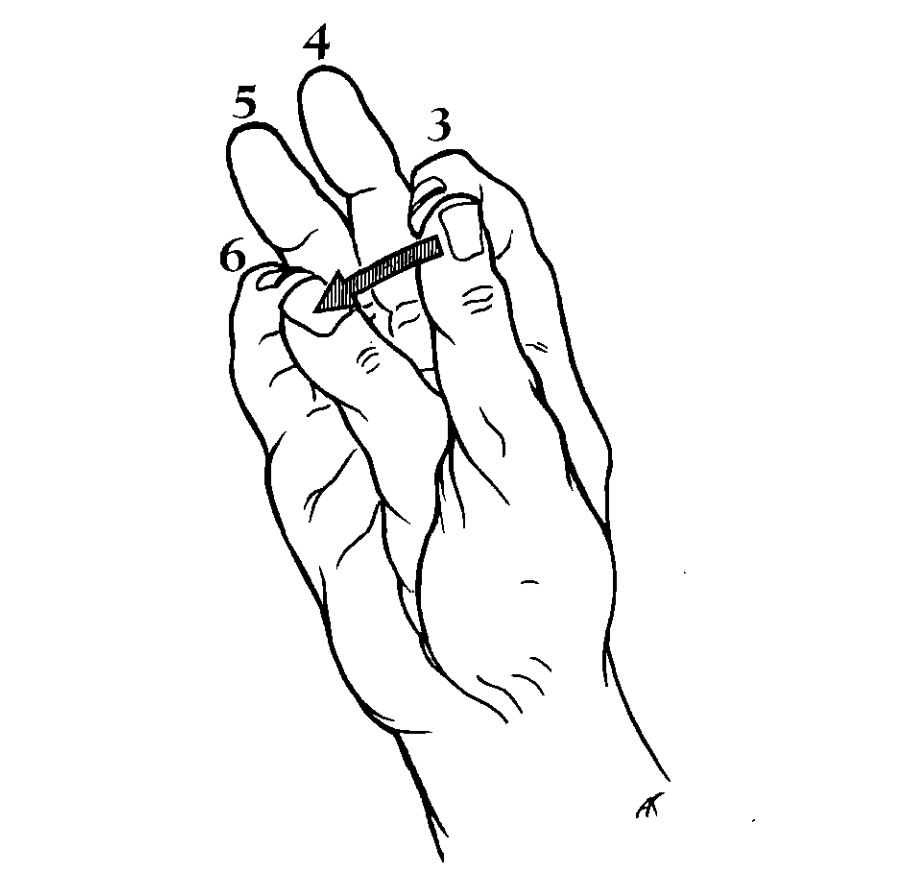
\includegraphics[height=40mm]{Images/kapandji_test.jpg}}\quad
%\subfigure[]{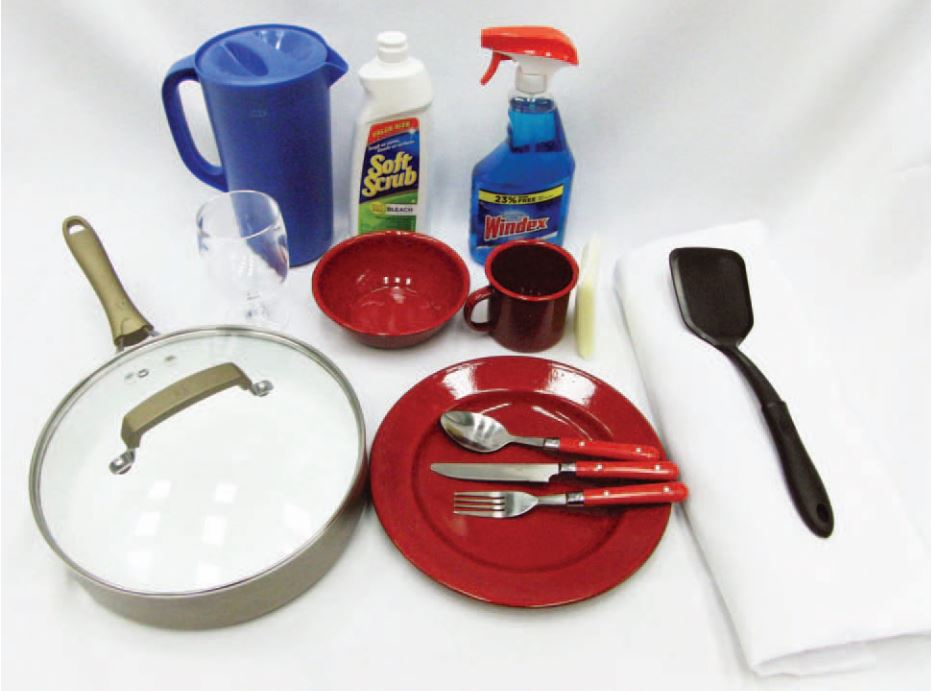
\includegraphics[height=40mm]{Images/ycb_kitchen.jpg}}\quad
\subfigure[]{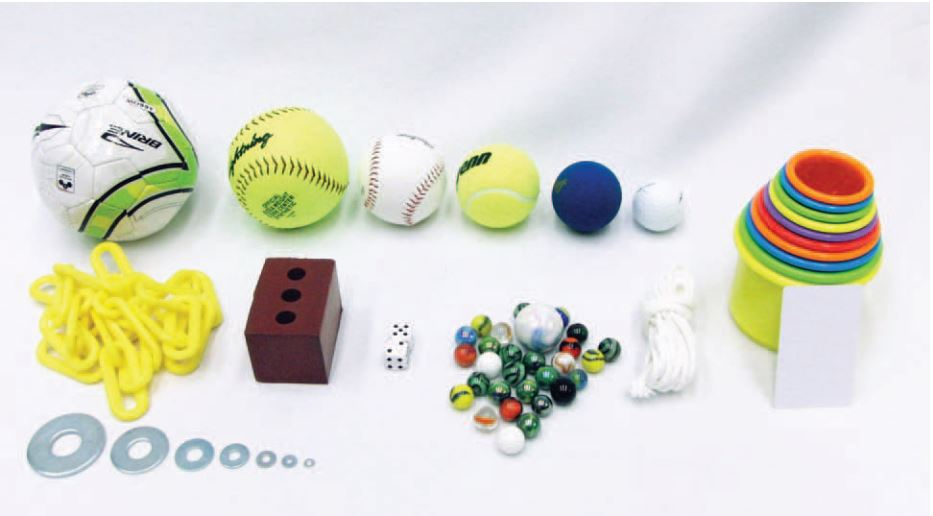
\includegraphics[height=40mm]{Images/ycb_shape.jpg}}\quad
%\subfigure[]{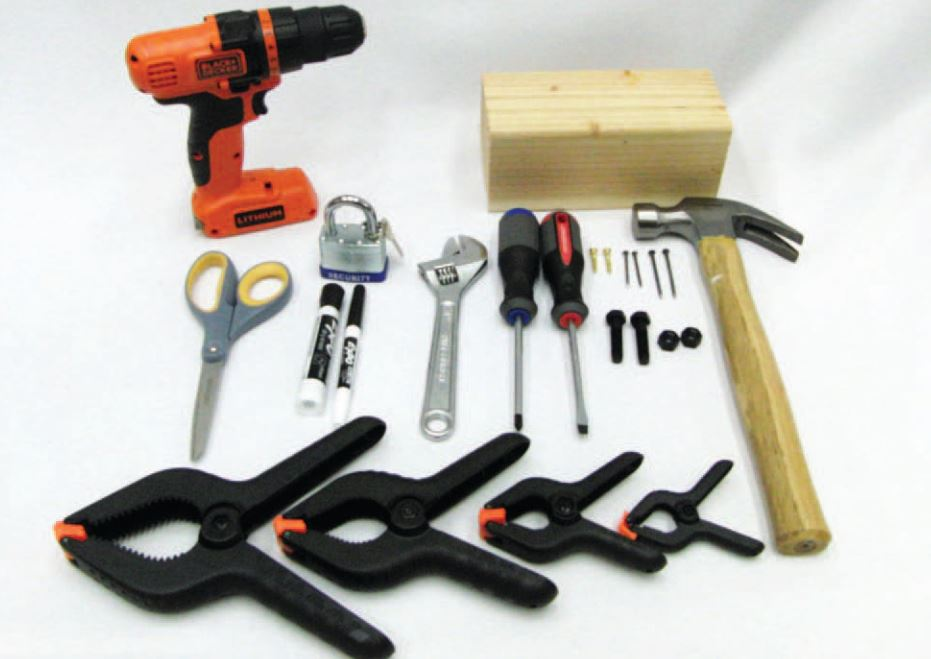
\includegraphics[height=40mm]{Images/ycb_tools.jpg}}\quad
%\subfigure[]{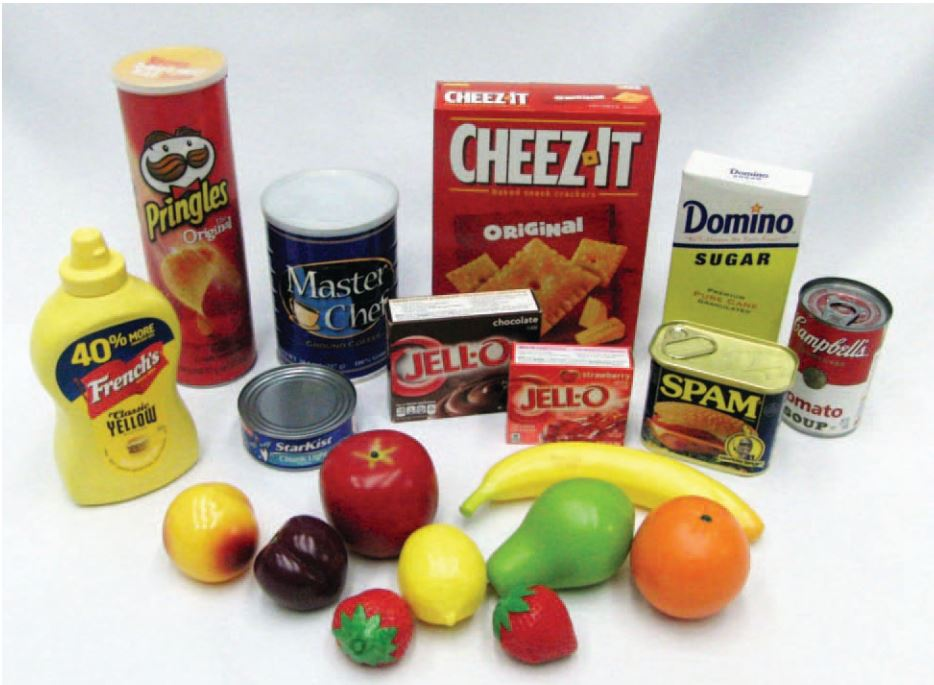
\includegraphics[height=40mm]{Images/ycb_food.jpg}}\quad
\caption[Other Testing]{\label{f:Other Testing} (a) Sketch of the opposing thumb test: In this particular test the thumb has to reach all the finger tips going from 3 to 6.(b) Extract of the YCB data-set with objects of different shapes.}
\end{figure}












